\documentclass[conc-doc]{subfiles}

\begin{document}
	
	\chapter[GPU/Parallel programming]{GPU/Parallel programming}
	\label{ch:gpuprogramming}

\doquote{9cm}{35pt}{6cm}{8cm}{9.2cm}{footnotesize}{Time to wake up\\Refill new destiny\\Through this}{The Whitest of Lies from Prototype by NeuroWulf (2005)}


Concurnas has built in first class citizen support for programming GPUs and associated parallel computing constructs. GPU's are massively data parallel computation devices which are perfect for solving SIMD (single instruction, multiple data) and normally CPU bound problems. Compared to a single CPU core algorithm implementation, in solving a computation bound problem, it is common to be able to obtain up to a 100x speed improvement (two orders of magnitude) when using a GPU! And this is with a far reduced energy and hardware cost per gigaflop relative to CPU based computation. All modern graphics cards have a built in GPU and there exist dedicated GPU computation devices. In fact some of the world's leading supercomputers achieve their parallelization through the use of dedicated GPU hardware. With Concurnas this power is your as well.

Support is provided via interfacing to OpenCL - an excellent multiplatform API for GPU computing. OpenCL is supported by the big three GPU manufacturers - NVidia, AMD and Intel. However, even with conventional, raw OpenCL (or any GPU computing platform for that matter) one must write a lot of boilerplate code and perform a lot of non work related management in order to get computation done on the GPU. A such, authoring large applications can be an intimidating prospect. With Concurnas you will see that this boilerplate code is minimized, allowing the developer to focus on solving real business problems. Additionally there is no need to learn (and have to paradigm shift into) C or C++ which is the native language used by OpenCL for expressing parallel functions on the GPU as functions marked as parallel in Concurnas are automatically translated into a form understandable by the GPU/OpenCL. GPU computing is for everyone.

The helper classes associated with GPU computing are a part of the core Concurnas API. This can be found here.

What follows is a practical guide covering the key components of GPU computing with Concurnas.

\section{Prerequisites}
In order to make use of the Concurnas GPU parallel programming solution the following prerequisites must be satisfied:

\begin{itemize}
	\item Access to at least one OpenCL ready GPU on one's computation machine (almost all modern graphics cards support this)
	\item OpenCL compatible driver compliant to at least version 1.2 of OpenCL for said GPU(s). Consult your graphics card manufacturer for support for details on this.
\end{itemize}


Concurnas enables parallel computation on GPU's, FPGA accelerators and conventional CPUs. Although OpenCL natively supports execution on the CPU, we do not encourage use of this in Concurnas for solving anything but strictly data based parallel problems.

To see if one has access to any GPU devices one can use the \lstinline{getGPUDevices} command as part of the GPU API:

\begin{lstlisting}
From com.concurnas.lang import gpus

gps = gpus.GPU()
gpudevices = gps.getGPUDevices()
firstDevice = gpudevices[0]
deviceDetails = firstDevice.toString()

//deviceDetails == NVIDIA CUDA: [GeForce GTX 570]
\end{lstlisting}

Note that \lstinline{com.concurnas.lang.gpus} is an auto import, therefore it is not necessary to explicitly import \lstinline{gpus}, and we shall cease to do so in the subsequent examples.

Note that a machine may have more than one GPU (in fact this is common with machines having integrated graphics processors either on the motherboard or CPU - often being Intel HD graphics). But, if no GPU devices are available it can be useful for some problems to 'fall back' on to CPU based computation. The interface/compute model is the same and one will still obtain the advantages of the SIMD instruction set whilst processing on the CPU which is quicker for data parallel problems than the alternatives provided in Concurnas (which are more oriented towards task parallelism). One can select the CPU's available on one's machine via the \lstinline{getCPUDevices}, example:

\begin{lstlisting}
def chooseGPUDeviceGroup(gpuDev gpus.DeviceGroup[], cpuDev gpus.DeviceGroup[]) gpus.Device {
	if(not gpuDev){//no gpu return first cpu
		cpuDev[0]
	}else{
		for(grp in gpuDev){
			if('Intel' not in grp.platformName){
				return grp
			}
		}
		gpuDev[0]//intel device then...
	}
}

gps GPU = gpus.GPU()
deviceGrp gpus.DeviceGroup= chooseGPUDeviceGroup(gps.getGPUDevices(), gps.getCPUDevices())
device gpus.Device = deviceGrp.devices[0]
\end{lstlisting}

In the above example we choose the first non Intel based GPU, failing that we fall back to returning the first CPU device available.

We can examine the capabilities of both the device group and the individual devices of which it composes by calling the get methods of interest on the objects. Here we just look at an example summary for both:

For the DeviceGroup:
\begin{lstlisting}
gps = gpus.GPU()
deviceGrp = gps.getGPUDevices()[0]

summary = deviceGrp getSummary()
/*
summary => 
Device Group:   NVIDIA CUDA: [GeForce GTX 570]
OpenCL Version: OpenCL 1.2 CUDA 9.1.84
Vendor:         NVIDIA Corporation
Extensions:     cl_khr_global_int32_base_atomics ...
*/
\end{lstlisting}

For an individual device:
\begin{lstlisting}
gps = gpus.GPU()
deviceGrp = gps.getGPUDevices()[0]
device = deviceGrp.devices[0]

summary = device getSummary
/*
summary => 
Device:                     GeForce GTX 570
Vendor:                     NVIDIA Corporation
Address Bits:               64
Available:                  true
Compiler Available:         true
Little Endian:              true
Error Correction Support:   false
Global Memory Size:         1.3 GB
Local Memory Size:          48.0 kB
Compute Units:              15
Clock Frequency:            1560
Constant Args:              9
Constant Buffer Size:       64.0 kB
Max Memory Allocation Size: 320.0 MB
Param Size:                 4352
Max Work Group Size:        1024
Max Work Item Sizes:        [1024 1024 64]
Base Address Align:         4096
Data Type Align Size:       128
Profiling Timer Resolution: 1000
Type:                       CL_DEVICE_TYPE_GPU
Vendor ID:                  4318
OpenCL Version:             OpenCL 1.1 CUDA
Driver Version:             391.35
Extensions:                 cl_khr_global_int32_base_atomics...
*/
\end{lstlisting}

\subsection{Code Portability}
When working with ordinary Concurnas code operating on general purpose CPUs, the computing environment and how one codes for it is assumed to be highly homogeneous. I.e. it's rare that one need to consider the clocks speed, amount of L1/L2 cache one's cpu has, or even the amount of RAM available for operation, generally speaking these things are automatically optimized/can be assumed as being adequate for ones software to run. Additionally, one does not need to adapt ones code to optimize for different CPU architectures/RAM configuration etc, this is something which the compiler/virtual machine takes care of. 

However, when one is working with GPUs, although there are many optimizations in place as part of the compilation process (e.g. optimal opcode generation, register allocation etc) the decisions required in order to optimally solve a problem on a GPU are generally left for the developer to optimize for, and if one is not diligent, one can write code which is not very portable/optimal for the range of GPUs one's code is run on. There are some properties referenced above which are of particular interest insofar as code portability is concerned, which generally need to be factored in in ones software:

\begin{itemize}
	\item \textbf{Address Bits} - This indicates whether the GPU is operating in a 32 or 64 bit environment. Determines the size of the \lstinline{size_t} primitive type. In order to assist with portability between 32 and 64 bit environments the \lstinline{size_t} primitive type - 32 bits (4 bytes being an \lstinline{int}) or 64 bits (8 bytes being a long) is provided. This is the type returned from functions such as \lstinline{get_global_id} and \lstinline{get_local_id}, \lstinline{sizeof} when used within gpu kernels and functions, is the datatype of pointers and is the type used to address arrays. This permits one to write code that is agnostic of whether one is operating in a 32 or 64 bit environment (though practically one can assume a 64 bit environment in most cases).
	\item \textbf{Local Memory Size} - This is the amount of memory per compute unit which is accessible to a work group (collection of parallel work items) running on it, this memory can be used as a limited shared cache between the work items in a work group.
	\item \textbf{Global Memory Size} - Note that GPUs usually have far less available to them on an individual basis than our host.
	\item \textbf{Max Memory Allocation Size} - Not only are we limited to the Global Memory Size, but chunks of memory may be no larger than this value. This is often a value one must consider when designing an algorithm for portability, and different GPUS often have different max allocation sizes.
	\item \textbf{Max Work Item Sizes} - When designing an algorithm which uses local memory, one must be cognizant of these values.
\end{itemize}

\section{Events}
It is advantageous for computation on the GPU to take place on an concurrent basis, both for performance reasons - in allowing the GPU to reorganise execution, and for practical reasons - as we can move data to, from and between gpu's (a relatively slow operation) at the same time as they are performing execution, thus enabling us to create mini pipelines of work for our GPU, always keeping it busy, maximising throughput.

In Concurnas we make use of OpenCL events to support control of asynchronous computing on the GPU. These are wrapped within refs and exposed as GPURef's. Many of the core GPU operations operate on an asynchronous, non blocking basis: reading, writing and copying data between the GPU and program execution.

GPURefs have their status set upon completion of the task which created them.

The typical workflow of execution involves first copying data to the gpu, performing execution, and then copying back the result to heap managed memory. We can wait, via the /await/ keyword, on the GPURefs returned from the data writing call to ensure that execution only begins after data copying is complete, similarly, we can wait on the GPURef returned from execution before continuing to copy the result to main memory. Following on from our previous example:

\begin{lstlisting}
intoGPU1 = device.makeOffHeapArrayIn<int[]>(int[].class, 10)
copyComplete boolean:gps.GPURef = intoGPU1.writeToBuffer([1 2 3 4 5 6 7 8 9 10])
await(copyComplete)
//rest of program will execute only when copyComplete has been set..
got = inoutGPU.readFromBuffer()
\end{lstlisting}

In the above example, had we not waited for the \lstinline{copyComplete} ref to complete, the \lstinline{readFromBuffer} call may have returned an unexpected result. So by explicitly waiting we are ensuring consistency.

There is a way to perform the above synchronization which is generally preferred from a performance and elegance of code perspective. All the non blocking GPU operations take a vararg of GPURef's to wait for before continuing execution:

\begin{lstlisting}
intoGPU1 = device.makeOffHeapArrayIn<int[]>(int[].class, 10)
copyComplete boolean:gps.GPURef = intoGPU1.writeToBuffer([1 2 3 4 5 6 7 8 9 10])
got = inoutGPU.readFromBuffer(copyComplete)//readFromBuffer will execute when coyComplete has been set
\end{lstlisting}

In the above example the blocking of the readFromBuffer call will take place within the OpenCL framework. Generally speaking this is the preferred method of synchronization as the control takes place closer to the hardware and the code is easier to write (at least in omitting the explicit call to await).

If one forgets to capture the resultant GPURef from an asynchronous, non blocking GPU operation, then the operation will turn into a blocking one as the calling code will wait for the resulting GPURef to be set. This is because all the asynchronous non blocking GPU operations are marked with the \lstinline{@com.concurnas.lang.DeleteOnUnusedReturn} annotation.

\section{Data transference}
\subsection{Buffers}
Before we can perform calculations on the GPU we must first copy data to our GPU device. We can work with both scalar values (single values) and n dimensional arrays. Data must be of type either: primitive or boxed primitive (Integer, Character etc). We must first create an appropriate buffer to work with the data on the GPU, this is a blocking operation:

\begin{lstlisting}
singl gpus.GPUBufferInputSingle = device.makeOffHeapArrayInSingle<int>(int.class)
\end{lstlisting}

Here, single has been created as an In buffer, allowing us to copy data into it only. Single and n dimensional array buffers can be created as either:

\begin{itemize}
	\item \textbf{In}: permitting only writing of data to them, most often used for arguments to kernels (makeOffHeapArrayInSingle/makeOffHeapArrayIn)
	\item \textbf{Out}: Permitting only reading of data from them, useful for results of kernels (makeOffHeapArrayOutSingle/makeOffHeapArrayOut)
	\item \textbf{Mixed}: Permitting both reading and writing of data. (makeOffHeapArrayMixedSingle/makeOffHeapArrayMixed)
\end{itemize}  

It is advised that one chooses from the above types of buffer carefully, as it allows the GPU to optimize memory access.

The reified method local generic type argument is used in order to determine the size of the underlying data allocation space on the GPU.

Let's now create some n dimensional arrays on the GPU:

\begin{lstlisting}
ar gpus.GPUBufferInput = device.makeOffHeapArrayIn<int[]>(int[].class, 10)
mat gpus.GPUBufferInput = device.makeOffHeapArrayIn<int[2]>(int[2].class, 2, 4)//2 by 4 matrix
\end{lstlisting}

Here we are creating both an array (ar) and a matrix (mat). Note how we must specify the dimensionality of the structure by populating the second argument of the method (which is a vararg) with its dimensions.

Normally, for n dimensional arrays, Concurnas uses Iliffe vectors (wikipedia link), but when working on the GPU, memory is organized in a serial manner. In practice this means is that n dimensional (where n> 1) arrays cannot be irregular in shape if you wish to correctly work with them on the gpu.

\subsection{Writing, Reading Data}
All of the commands used to read, write and copy data to GPU buffers are non blocking and will return a GPURef for synchronization. They also take a list of GPURefs to wait for completion for as a final vararg.

Let us write some data to an In Buffer:

\begin{lstlisting}
ar gpus.GPUBufferInput = device.makeOffHeapArrayMixed<int[]>(int[].class, 10)
copyComplete boolean:gps.GPURef = ar.writeToBuffer([1 2 3 4 5 6 7 8 9 10])
\end{lstlisting}

We can pass any n dimensional array of the buffer type to an In or Mixed buffer using the \lstinline{writeToBuffer} method. However, since the data is flattened for purposes of execution on the gpu, but we must ensure that the data passed is of equal size to that of the buffer otherwise a runtime exception will be thrown. For instance, it would be acceptable to for a 1 dimensional int array of 10 elements to be passed to a 2 dimensional array (matrix) buffer with 2 x 5 dimensionality as the data size is the same (\lstinline{10 ==  2 * 5 => 10} entries).

We can read from a buffer as follows:
\begin{lstlisting}
result int[] = ar.readFromBuffer(copyComplete)
\end{lstlisting}

Note above by passing in the \lstinline{copyComplete} ref we are waiting for the write operation to first complete.

Single buffers are even easier to work with:
\begin{lstlisting}
ar gpus.GPUBufferInput = device.makeOffHeapArrayMixed<int>(int.class)
copyComplete boolean:gps.GPURef = ar.writeToBuffer(99)
result int = ar.readFromBuffer(copyComplete)
//result = 99
\end{lstlisting}

\subsection{Copying Data}
We can copy data from an Out or Mixed buffer to a In or Mixed buffer using \lstinline{copyToBuffer}:
\begin{lstlisting}
intoutGPU1 = device.makeOffHeapArrayMixed<int[]>(int[].class, 10)
intoutGPU2 = device.makeOffHeapArrayMixed<int[]>(int[].class, 10)
c1 := intoutGPU1.writeToBuffer([1 2 3 4 5 6 7 8 9 10])

g1 := intoutGPU1.copyToBuffer(intoutGPU2, c1)
//intoutGPU2 now contains a copy of the data asigned to intoutGPU1
\end{lstlisting}

The above copy mechanism can be used in order to copy non overlapping regions of data inside the same buffer.

\subsection{Writing, Reading and Copying subregions}
We can copy subregions of data to and from as well as between buffers using the \lstinline{[a ... b]}, \lstinline{[a .. ]} and \lstinline{[ ... b]} syntax and via additional arguments to the \lstinline{copyToBuffer} method. When using the \lstinline{[ ... ]} syntax since we have no way of capturing the resultant GPURef of the write or read operation, the caller will block implicitly until this is returned, and will call delete on the GPURef object freeing the memory used for it on the GPU.

\begin{lstlisting}
intoutGPU1 = device.makeOffHeapArrayMixed<int[]>(int[].class, 20)
//intoutGPU1 is inialized with all 0's

intoutGPU1[5 ... 8] = [66 55 44]//blocking operation
subWrite := intoutGPU1.subAssign(15, 18, [66 55 44])//non blocking operation

await(subWrite)

result1 = intoutGPU1[5 ... 8]//blocking subread
result2 := intoutGPU1.sub(15 18)//non blocking subread

await(result2)
\end{lstlisting}

The other variants of subregion are intuitive.

When copying between regions we can add additional arguments to the \lstinline{copyToBuffer} method:
\begin{lstlisting}
intoutGPU1 = device.makeOffHeapArrayMixed<int[]>(int[].class, 10)
intoutGPU2 = device.makeOffHeapArrayMixed<int[]>(int[].class, 10)
c1 := intoutGPU1.writeToBuffer([1 2 3 4 5 6 7 8 9 10])

g1 := intoutGPU1.copyToBuffer(intoutGPU2, 2, 4, 2, c1)
\end{lstlisting}

Here, we are copying two items from \lstinline{intoutGPU1} into the 2nd index of \lstinline{intoutGPU2}.

\section{sizeof}
It can be useful to know how many bytes of memory a structure will take up on the GPU. To this end a qualifier can be specified to the \lstinline{sizeof} keyword as follows:

\begin{lstlisting}
myArray = [0 1 2 3 4 5 6 7 8 9]
size = sizeof<gpus.gpusizeof> myArray 
//myArray == 40 bytes
\end{lstlisting}

\section{Kernels and functions}
Kernels are the core which drive our execution on the GPU. The compute model for kernels does have a number of differences relative to non gpu Concurnas code which one needs to be aware of in order to derive maximum value from them.

Here is an example kernel for simple matrix multiplication\footnote{Those readers familiar with the intricacies of GPU optimization will recognize this as a naive, unoptimized, implementation. This is intentional and we shall cover some details of Kernel optimization later.} with its conventional, non GPU counterpart on for comparison:

%begin-twoCol
\noindent\begin{minipage}{.45\textwidth}
	\begin{lstlisting}[caption=GPU kernel,frame=tlrb]{Name}
gpukernel 2 matMult(wA int, wB int, global in matA float[2], global in matB float[2], global out result float[2]) {
	globalRow = get_global_id(0) // Row ID
	globalCol = get_global_id(1) // Col ID
	
	value = 0f;
	for (k = 0; k < wA; ++k) {
		value += matA[globalCol * wA + k] * matB[k * wB + globalRow];
	}
	
	// Write element to output matrix
	result[globalCol * wA + globalRow] = value;
}
\end{lstlisting}
\end{minipage}\hfill
\begin{minipage}{.45\textwidth}
	\begin{lstlisting}[caption=CPU equivilent,frame=tlrb]{Name}
def matMult(M int, N int, K int, A float[2], B float[2], C float[2]) {
	for (m=0; m<M; m++) {
		for (n=0; n<N; n++) {
			acc = 0.f
			for (k=0; k<K; k++) {
				acc += A[k][m] * B[n][k]
			}
			C[n][m] = acc
		}
	}
}
\end{lstlisting}
\end{minipage}
%end-twoCol

The GPU kernel is only executable on a device as par below. Kernels cannot be executed via normal function invocation. GPUs operate on a single instruction, multiple data basis, thus unlike the non gpu code on the right, the two outermost for loops are not required as the kernel is executed in parallel on the cores of the GPU device executing it. 

We can use something like the following in order to execute the kernel on the GPU (assuming we have already selected a device):
\begin{lstlisting}
inGPU1 = device.makeOffHeapArrayIn(float[2].class, 2, 2)
inGPU2 = device.makeOffHeapArrayIn(float[2].class, 2, 2)
result = device.makeOffHeapArrayOut(float[2].class, 2, 2)

c1 := inGPU1.writeToBuffer([1.f 2.f ; 3.f 4.f])
c2 := inGPU2.writeToBuffer([1.f 2.f ; 3.f 4.f])

inst = matMult(2, 2, 2, inGPU1, inGPU2, result)//create a 'kernel' object from our gpukernel
compute := device.exe(inst, [2 2], c1, c2)//execute kernel on device, with 2 x 2 (4) work items, whilst waiting for c1 and c2 (operations to write to gpu) to complete
 ret = result.readFromBuffer(compute)//read result from output buffer, whilst waiting for gpu to finish execution of our kernel
\end{lstlisting}

We shall now look in detail at what is taking place above...

\subsection{Work Items}
The memory/execution model for OpenCL exposed within Concurnas is as follows:

\begin{figure}[H]
	\centerline{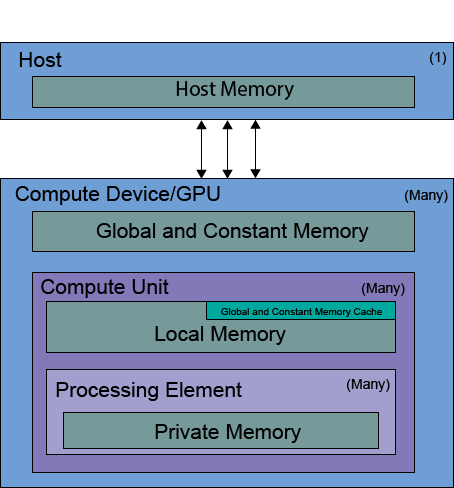
\includegraphics[width=.9\textwidth]{images/gpu-memModel.png}}
	\caption{Memory/execution model for OpenCL exposed within Concurnas}
	\label{fig:memModel}
\end{figure}


As shown in \ref{fig:memModel}, each host machine may have many Compute devices, each made up of multiple compute units, themselves holding multiple processing elements.

When we execute Kernels, they are executed as work items in parallel across processing elements of the compute units (as work groups) on the GPU device(s) we invoke them on. Processing elements have their own private memory space where they store registers etc, and they have access to the local memory of the compute unit they are a part of as well as global memory. Access to these memory spaces for processing elements executing work items is exponentially slower the further one moves away from the processing element - hence, private memory access is the quickest, then local memory and then global memory, however, the amount of memory at each level available is inversely proportional to the locality. We have some respite when accessing repeated elements of global memory however as a portion of local memory (normally 16Kb of the 64Kb total) is dedicated to caching global and constant memory.

As we have already seen, interaction between host and compute device memory is governed via the use of buffers. Moving data from the host to the GPU is a relatively slow operation, in fact, generally speaking reading data from a GPU is approximately 10x slower than writing data. This must be factored into the design of most systems which take advantage of the GPU.

Each kernel instance is able to determine which unique work item it is by invoking the \lstinline{get_global_id} auto imported gpu function.The most common way to operate on data in parallel on the gpu is then to take this identifier and use it to select a section of data to operate on. For example, here is a very simple kernel adding two 1 dimensional arrays together, interacting with both global and constant memory:

\begin{lstlisting}
gpukernel 1 addtwo(constant A int[], constant B int[], global out C int[]){
	id = get_global_id(0)
	C[id] =A[id] + B[id]
}
\end{lstlisting}

Each work item here is operating on one item of data (one from A, one from B and one written to C), but, as par our matrix multiplication example above, work items may address more than one item of data.

We generally do not need to concern ourselves with the way in which Kernels are mapped to compute units and then individual work items (as this is automatically handled) unless we are looking at optimizing code - which we shall examine later.

\subsection{Kernel dimensions}
Most GPU parallelism is performed on n-dimensional array data. N-dimensional arrays in Concurnas kernels are always flattened to 1 dimensional arrays. This is performed implicitly when data is copied into a GPU Buffer. Likewise, when data is copied out of a GPU buffer, it is converted back into its n dimensional form. Given this flattening of n dimensional array data, navigation around the array space is thus performed via arithmetic, with consideration for the dimensionality of the arrays.

In order to assist with this array navigation, kernels must specify a dimension parameter between 1 and 3 (set to \lstinline{2} in the above example). One can consider that for the case of a 2 dimensional kernel, the execution is performed as a matrix. Thus a call to \lstinline{get_global_id(0)} provide an x axis, and \lstinline{get_global_id(1)} will a y axis reference (note if the kernel dimensionality was set to 3 then we would be able to call, \lstinline{getGlobalId(3)} to return a z axis reference). If the kernel were specified as a 1 dimensional kernel then only a \lstinline{getGlobalId(0)} call would be valid.


%begin-twoCol
\begin{figure}[H]
	\sidebyside{
		Conventional storage on the heap\\
		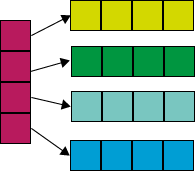
\includegraphics[width=.45\textwidth]{images/gpu-heap1.png}\\
		\lstinline{arr[n][m]}
	}
	{
		Storage on the GPU\\
		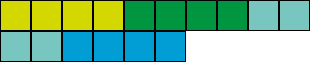
\includegraphics[width=.45\textwidth]{images/gpu-heap2.png}\\
		\lstinline{arr[n*4 + m]}
	}
	\caption{A 4 x 4 matrix allocated on the heap and the same matrix on the GPU.}
	\label{fig:memAllocation}
\end{figure}
%end-twoCol

In \ref{fig:memAllocation} we see an example of this effect on a 4x4 matrix and how on these are addressable conventionally and on the GPU.

\subsection{Kernel arguments}
The syntax for kernel arguments is slightly more involved than for normal function definitions in Concurnas:

\begin{center}
	\lstinline{annotations? (global|local|constant)? (in|out)? (val|var)? name primitive_type}
\end{center}

All kernel parameters must be of primitive time or boxed equivalent (Integer, Float etc). Any kernel parameters may be marked as either: global, local or constant or without a qualifier - those that are are treated as pointers (See Pointers ) within the body of the function:

\begin{itemize}
	\item \lstinline{global} - The parameter value is held within the global memory space, it must be a pointer type (function parameters are automatically converted to this form)
	\item \lstinline{local} - The parameter value is held within the local memory space specific to the compute unit the processing element operating the work item instance of the current kernel resides within. Note that it is limited in size to generally no larger than 64 Kb.
	\item \lstinline{constant} - The parameter is a constant. Changes cannot be made to the value. The amount of constant space on a gpu is limited and implementation specific (see the device parameter: Constant Args and Constant Buffer Size above), though usually it's 64Kb.
	\item BLANK - Indicates that the parameter is private to the kernel instance and may not be shared amongst work group items. Changes can be made but they are not visible outside of the work item.
\end{itemize}

Kernel parameters marked as global may optionally be marked with the type of buffer capability they expect. This further enhances the type safety provided by Concurnas when working with GPU's:

\begin{itemize}
	\item \lstinline{in} - indicating that only an in or mixed buffer may be used as an invocation argument.
	\item \lstinline{out} - indicating that only an out or mixed buffer may be used as an invocation argument.
	\item BLANK - indicating that any type of buffer (in, out or mixed) is permissible as an invocation argument.
\end{itemize}

Kernel arguments may be specified as arrays of dimensionality greater than 1, however, within the kernel itself these are flattened to one dimension, as discussed in the Kernel dimensions section above, are only addressable as such. Additionally they are useable only as pointers.

\textbf{Type erasure}. Due to the fact that generic types are erased at runtime it is not possible for Concurnas to differentiate between gpukernel function signatures differing by global/local/constant parameter qualification or in kernel dimensions. Hence the following three definitions are ambiguous:
\begin{lstlisting}
gppukernel 1 kfunc(global A int[]){... }
gppukernel 1 kfunc(local A int[]){... }//ambiguous
gppukernel 2 kfunc(global A int[]){... }//ambiguous
\end{lstlisting}

But Concurnas is able to differentiate between signatures differing in terms of in/out parameter qualification. Hence the following is not ambiguous:
\begin{lstlisting}
gppukernel 1 kfunc(global in A int[]){... }
gppukernel 1 kfunc(global out A int[]){... }//NOT ambiguous!
\end{lstlisting}

\subsection{Calling functions from kernels}
One is not limited just to executing code within kernels. Kernels may invoke other kernels (with matching kernel dimensions), built in utility functions as well as defined callable functions declared as gpudef:

\begin{lstlisting}
gpudef powerPlus(x int, raiseto int, plus int) => (x ** raiseto ) + plus 
\end{lstlisting}

As with kernels, input parameters may be marked as either global, local or constant or without a qualifier, they cannot be invoked like normal Concurnas functions, are type erased and they are subject to the same restrictions in their definition, as described below. \lstinline{gpudef} functions cannot be called by ordinary Concurnas code.

There are a number of essential and useful built in utility functions which are auto included for all gpu kernels and gpu functions. Two common and essential ones are:
\begin{itemize}
	\item \lstinline{get_global_id(dim int) int} - returns the global id for the dimension specified
	\item \lstinline{get_local_id(dim int) int} - returns the local id for the dimension specified.
\end{itemize}

The full list of utility functions can be found at: \lstinline{com.concurnas.lang.gpubuiltin.conc}

\subsection{Stub functions}
Sometimes, particularly in the cases where one has existing opencl C99 compliant OpenCL C code to use in Concurnas, it can be useful to define functions as stubs and reference in this code. We can achieving this in two ways via the use of the \lstinline{com.concurnas.lang.GPUStubFunction} annotation as follows:

\textbf{Explicit source}. The source parameter of the annotation consumes a String holding the C99 compliant OpenCL c code to load in place of the function definition when called by the GPU. This is a useful technique for expressing smallish blocks of code:

\begin{lstlisting}
@GPUStubFunction(source="float plus(float a, float b){ return a + b;}")
gpudef plus(a float, b float) float
\end{lstlisting}

\textbf{Source files}. The sourcefiles parameter of the annotation consumes an array of Strings referencing the files holding the C99 compliant OpenCL c code to use in place of the function definition when called by the GPU. The file referenced may be absolute or relative to the working directory:

\begin{lstlisting}
@GPUStubFunction(sources=['./cpucode.cl', './gpuutilCode.cl'])
gpudef plus(a float, b float) float
\end{lstlisting}

The two methods above can be used together, i.e. it's possible to define both explicit source code and files to import. The Annotation may be attached to regular functions (which may optionally be declared abstract), gpudef functions and gpukernels (which must be declared abstract).

It's also possible to use neither explicitly defined source code or reference any source files. In this case Concurnas will assume that the dependant code has been included in a explicit source or source file definition specified in a different GPUStubFunction reference.

Note that Concurnas assumes that the source code provided is correct, i.e. the enhanced type safety which Concurnas provides at compile time for GPUs cannot be provided with stub functions. However, runtime safety is still provided, and invalid code within a kernel chain will be flagged in a GPUException upon invocation.

\subsection{Recursion}
We are not permitted to make use of recursion when defining gpu kernels and functions, either directly or indirectly. However, it's often rare that an algorithm genuinely requires recursion, beyond satisfying code aesthetics, in order to solve a problem. Often recursive solutions to problems can be rewritten in a non recursive, though less graceful, matter. Let us look at a classic recursive solution to the fibonacci series generation problem, in classical Concurnas on the left and in Parallel gpu Concurnas code on the right:

%begin-twoCol
\noindent
\begin{minipage}{.45\textwidth}
	\begin{lstlisting}[caption=Classical Concurnas code,frame=tlrb]{Name}
def fib(n int) long{
	if(n == 0){
		return 0
	}elif(n <== 2){
		return 1
	}else{
		return fib(n-2) + fib(n-1)
	}
}





.
\end{lstlisting}
\end{minipage}\hfill
\begin{minipage}{.45\textwidth}
	\begin{lstlisting}[caption=Parallel GPU Concurnas code,frame=tlrb]{Name}
gpudef fib(n int) long {
	if(n == 0){
		return 0
	}elif( n <== 2){
		return 1
	}else{
		r = 0L; n1 = 1L; n2 = 1L       
		for(i = 2; i < n; i++){
			r = n1 + n2
			n1 = n2
			n2 = r
		}
		return r
	}	
}
\end{lstlisting}
\end{minipage}
%end-twoCol

\subsection{Function overloading}
Although Concurnas will permit us to define more than one version of a function in an overload manner (same name, different signature), only one version of that overloaded function may be referenced in an execution of a kernel. This restriction is checked for via a compile time and runtime check.

\subsection{Kernel and function variables}
Similar to kernel and function parameters, variables may be qualified with \lstinline{local} or \lstinline{global}. E.g.:
\begin{lstlisting}
local xyz3 int[] = [1 2 3] //an array defined in local memory
\end{lstlisting}

Variables qualified as \lstinline{constant} may only be created at the top level of the code outside of any gpu kernels or functions. They may be referenced across multiple gpu kernels or functions. For example:

\begin{lstlisting}
constant fixedInc = 100

gpukernel 1 incrementor(global in A int[], global out B int[]) {
ida = get_global_id(0) 
B[ida] = A[ida] + fixedInc
}
\end{lstlisting}

There are a some additional caveats concerning qualified variables one must note:

\begin{itemize}
	\item Constant variables cannot be re-assigned to once they have been declared.
	\item Global variables may be of pointer type only.
	\item By qualifying variables in the above manner, we are indicating to our GPU that we wish the value of the variable to persist within the const, local or global memory space of the GPU. As such, once a variable has been qualified as say, global, it cannot be reassigned to a non global (practically just local) variable, as they are different physical memory spaces on the GPU.
\end{itemize}

\subsection{Kernel/function restrictions}
When it comes to writing code to run on the gpu, whether it be kernels or functions, there are a number of restrictions in terms of what components of Concurnas can be used both when defining and using them. Some of these have already been elaborated. The full list is as follows:

\begin{itemize}
	\item GPU Kernels and functions must be declared as functions. They may not be class methods or be nested in any way.
	\item Only GPU Kernels and functions may only invoke one another, they cannot invoke normal Concurnas functions. Non GPU Concurnas code may not directly invoke GPU Kernels or functions. (invocation from non GPU Concurnas code is described in the section below Invoking Kernels).
	\item The parameters of GPU Kernels and GPU functions must all:
	\begin{itemize}
		\item Be of primitive type (or boxed equivalent) and be of any array dimensionality (though inside the kernel this is flattened to one level if marked global, local or const)
		\item May not be varargs
		\item May not have default values
		\item May be marked as either global, local or constant or without a qualifier. If the parameter is qualified then it will be converted to a pointer within the body of the function. On invocation, will require a corresponding buffer object to be passed to it.
		\item May be marked with in or out to denote readwriteability.
	\end{itemize}
	\item GPU Kernels must return void.
	\item Variables declared outside the scope of a gpu kernel or gpu function must be declared val for them to be used inside.
	\item Recursion of GPU Kernels or GPU functions, either directly or indirectly is not supported.
	\item Overloading of GPU Kernels or GPU functions is not supported.
	\item The new operator may not be used - except for creating arrays.
	\item Arrays can only be created with dimensions expressed as constants\footnote{These are created on the stack and not the heap, unlike conventional arrays in Concurnas}.
	\item Kernels must have a dimensionality expressed of between 1 and 3.
	Note that Kernel parameters themselves may be natively of more than one dimension, when passed to a GPU buffer they will be implicitly flattened to one dimension as previously described.
\end{itemize}

Additionally, the following elements of Concurnas syntax/functionality may not be utilized:
\begin{itemize}
	\item Objects:
	\begin{itemize}
		\item Enumerations
		\item Direct or self returning dot operator
		\item Lambdas
		\item init blocks
		\item Method references
		\item \lstinline{&==} and \lstinline{&<>}
		\item Annotations
		\item The super keyword
		\item Local classes
		\item Nested functions
		\item Tuples
	\end{itemize}
	\item Object Providers
	\item Generics
	\item Pattern matching
	\item Exceptions:
	\begin{itemize}
		\item Try catch
		\item Throwing of exceptions
	\end{itemize}
	\item Compound statements:
	\begin{itemize}
		\item Break and continue returning a value
		\item Only \lstinline{for( ; ; ) } is valid, other variants of \lstinline{for} are not
		\item For and while blocks with else
		\item For and while blocks an index
		\item Compound statements which return a value (\lstinline{if}, \lstinline{while}, \lstinline{for} etc)
	\end{itemize}
	\item Concurrency/reactive computing:
	\begin{itemize}
		\item The await keyword (if you want to use this then barriers are probably the solution)
		\item Refs
		\item The changed keyword
		\item \lstinline{onchange, every, async}
		\item \lstinline{async, sync}
		\item Actors
		\item \lstinline{parfor, parforsync}
		\item Transactions
	\end{itemize}
	\item Arrays/Maps:
	\begin{itemize}
		\item Arrays of non constant size (e.g. \lstinline{new int[n]} where \lstinline{n} is a variable)
		\item Array default values
		\item The length parameter of an array is not exposed.
		\item List instantiation
		\item Empty arrays
		\item Maps
		\item Array pre/post and sublist range references
		\item Instantiated arrays outside of assignment statements
	\end{itemize}
	\item References to non constant module level, global, variables
	\item Other:
	\begin{itemize}
		\item The assert keyword
		\item Named parameters on function invocations
		\item \lstinline{@} copy
		\item The \lstinline{del} keyword
		\item offHeap data
		\item The \lstinline{in} or \lstinline{is} keywords
		\item the \lstinline{>>>} operator (\lstinline{<<} and \lstinline{>>} are ok)
		\item \lstinline{sizeof} with qualification. Normal \lstinline{sizeof} is ok
		\item string and regex declarations
		\item The \lstinline{with} keyword
		\item Language extensions
		\item Multi assign using an assignor other than \lstinline{=} or with \lstinline{global}/\lstinline{local}/\lstinline{constant} variables.
		\item The null safety related operators: safe call: \lstinline{?.}, elvis: \lstinline{?:} or not-null assertion: \lstinline{??}
	\end{itemize}
\end{itemize}

Concurnas handles the above restrictions at multiple levels in the programming and execution process by checking for them as part of the type system, during compilation time and finally at runtime. Unfortunately, for the C99 compatible C code expressed via stub functions, the restriction checking and error reporting, although comprehensive, is performed at runtime - which is of course not as convenient or safe as if it were to be performed exclusively at compile time.

\subsection{Invoking kernels}
Returning to our complete matrix multiplication example above:
\begin{lstlisting}
inGPU1 = device.makeOffHeapArrayIn(float[2].class, 2, 2)
inGPU2 = device.makeOffHeapArrayIn(float[2].class, 2, 2)
result = device.makeOffHeapArrayOut(float[2].class, 2, 2)

c1 := inGPU1.writeToBuffer([1.f 2.f ; 3.f 4.f])
c2 := inGPU2.writeToBuffer([1.f 2.f ; 3.f 4.f])

inst = matMult(2, 2, 2, inGPU1, inGPU2, result)//create a 'kernel' object from our gpukernel
compute := device.exe(inst, [2 2], c1, c2)//execute kernel on device, with 2 x 2 (4) work items, whilst waiting for c1 and c2 (operations to write to gpu) to complete
ret = result.readFromBuffer(compute)//read result from output buffer, whilst waiting for gpu to finish execution of our kernel
\end{lstlisting}

We first obtain the kernel by calling the gpukernel function like a normal function invocation, this will return a GPUKernel object which can be executed by a device. Global, local and constant kernel parameters must be satisfied with arguments that are buffers (inGPU1 and inGPU2 above). Unqualified arguments may point to non buffered variables, but note however that these are copied at invocation time to the GPU so it is advisable to keep these data structures small since as previously discussed, data transference is often the bottleneck in GPU work

Next we call exe on our chosen device. If this is the first time we have called the kernel on the device's parent device group, then the kernel will be compiled which takes a non epsilon amount of time. We must pass in an array, the product of which corresponds to the number of work items we wish to spawn in the number of dimensions (between 1 and 3 inclusive), corresponding to those required of our kernel. We may also optionally specify any local dimensions in the same way. Finally we can optionally pass in references to events to wait for completion of, in the above example we wait for the buffer write operations in events c1 and c2 to complete.

An GPURef object holding the execution completion event is returned from the exe method. Execution of a kernel is said to have completed one all of the work items have completed execution. As with buffer operations, kernel execution is a non blocking asynchronous operation, so we must wait on this object is appropriate.

\section{Profiling}
The Concurnas GPU implementation provides detailed profiling options. This is useful for both development, in enabling one to debug one's GPU code so as to determine how much time is spent performing certain operations, and for monitoring purposes. GPURef objects created from asynchronous non blocking gpu operations have a getProfilingInfo method, which returns an object of type GPUProfilingInfo class holding all the profiling information available:
\begin{lstlisting}
c1 := inGPU1.writeToBuffer([ 1 2 3 4 ])
copyduration = c1.getProfilingInfo().getWorkDuration()
summary = c1.getProfilingInfo().toString()
\end{lstlisting}

In the above example, the value returned from the getWorkDuration method call is a delta in nanoseconds (divide this by 1e6 to obtain a millisecond value).

\section{Pointers}
Since when working with GPUs we are working closer to the metal than ordinary Concurnas code, when writing gpu kernels and gpu functions we are afforded access to the use of pointers. These operate the same as pointers in low level languages such as C and C++ and can be very useful for defining programs to operates on the GPU or porting over existing code to operate within the Concurnas framework and not having to rely on GPUFunctionStubs (and the reduced amount of type safety stubs expose). Pointers are especially useful when working with subregions of global memory variables.

A pointer is a variable which contains the memory address of a different variable. We can have a pointer to any variable type. Pointer types are defined as follows:
\begin{center}
	\lstinline{ (*+)ordinaryType }
\end{center}

Example pointer types:
\begin{lstlisting}
*int //a pointer to an integer
*float//a pointer to a float
**int//a pointer to a pointer to an integer
***int//a pointer to a pointer to a pointer to an integer
\end{lstlisting}

The \lstinline{~} operator provides the address of a variable:
\begin{center}
	\lstinline{ ~variable }
\end{center}

We can use the \lstinline{~} operator in order to create pointers like this:
\begin{lstlisting}
normalVar int = 12
pnt *int  = ~normalVar //pointer holding the address of normalVar 
pnt2pnt **int = ~pnt //pointer holding the address of the pointer to normalVar 
\end{lstlisting}

The type upon which we apply the address \lstinline{&} operator must match that to which the pointer type refers. For example:
\begin{lstlisting}
aint = 12
afloat = 12.f

pnt1 *int = ~aint //ok int == int
pnt2 *int = ~afloat //error, type mismatch, int <> float
\end{lstlisting}

If we want to obtain the value pointed to by a pointer, we prefix the variable with the dereference operator /*/. We can prefix it for as many times as we require dereferencing:
\begin{lstlisting}
normalVar = 12
pnt  = ~normalVar 
pnt2pnt  = ~pnt 

//now for the dereferencing:

normalVarAgain int = *pnt 
aPointer *int = *pnt2pnt
normalVarOnceMore int = **pnt2pnt
\end{lstlisting}

In order to disambiguate pointer dereferencing from the multiplication operator, parentheses must be used:
\begin{lstlisting}
normalVar = 12
pnt  = ~normalVar 
pow2 = (*pnt) * (*pnt)
\end{lstlisting}

The dereferencing operation is similar for when we want to set the value pointed to by a of a pointer:
\begin{lstlisting}
normalVar = 12
pnt *int = ~normalVar 
*pnt = 99 //the variable normalVar now equals 99
\end{lstlisting}

\subsection{Pointers and Arrays}
Pointers and arrays in gpu kernels and gpu functions are two closely related concepts. We can set the value of a pointer to be the address of an array with element offset (remember, we count from 0) as follows:
\begin{lstlisting}
normalArray = [1 2 3 4 5]
pnt1  *int = ~normalArray[0] //pnt1 is set to the address of the first (start) element of the array
pnt2  *int = ~normalArray[1] //pnt1 is set to the address of the second element of the array
\end{lstlisting}

An especially useful feature of pointers to arrays (and strictly speaking, pointers in general) is the ability to perform pointer arithmetic and use them, syntactically, as one dimensional arrays:
\begin{lstlisting}
normalArray = [1 2 3 4 5]
pnt1  *int = ~normalArray[0]
pnt2  *int = ~normalArray[1]

//arithmetic...

pnt1++//pnt1 now points to the second entry in normalArray
avalue = *(pnt1+1)//avalue now equals the 3rd value from normalArray, 3
*(pnt2+1) = 100//set the 3rd value of normalArray to 100
extracted = pnt2[3]//obtain the 3rd value of normalArray, which is now 100
\end{lstlisting}

Multi dimensional arrays can be operated on in a similar way:
\begin{lstlisting}
myAr = new int[3, 4] //a matrix
myAr[0, 0] = 12
myAr[0, 1] = 14

pnt *int = ~myAr[0][0]//set pnt to point to the first value of the matrix
pnt += 1//pnt now points to the second value of the first row of the matrix

value = *pnt//value is now 14
\end{lstlisting}

\subsection{Array of pointers}
Sometimes it can be useful to make use of an array of pointers. This can be defined as follow:
\begin{lstlisting}
a = 44
b = 88
c = 23

pntc = ~c
arOfPnt *int[] = [~a ~b pntc]//array of pointers
*arOfPnt[1] = 99	//b now equals 88
\end{lstlisting}

\section{Local memory}
It is expensive to read and write to global memory, thus for algorithms involving a  high degree of spatial locality, using local memory can greatly improve processing time performance. This is achieved by essentially manually caching the data of interest to a work group (composed of a number of work items operating on processing units) within the local memory region specific to the compute unit work group. Here we will examine how this can be achieved.

Data that is in local memory is shared between all work items in a work group. Recall that compute units on a gpu execute the work items as part of a work groups on their processing elements. This interaction usually needs to be synchronised by using barriers. Work items in different work groups (resident therefore on different compute units) cannot share information via local memory - this has to be achieved via using global memory.

\subsection{Local Buffers}
We can specify local kernel parameters by qualifying them with \lstinline{local}. When doing so they must be satisfied with \lstinline{gpus.Local} buffers on kernel invocation as follows:
\begin{center}
	\lstinline{localBuffer = gpus.Local(long[].class, localItemSize)}
\end{center}

Essentially we are just providing the type and buffer size information. Local buffers provide no means to write into/out of them outside the GPU. This of course means that local kernel parameters may not be further qualified as being \lstinline{in out} parameters.

The amount of local memory available to a work group executing on a compute unit is limited - generally it is no more than 64Kb, to be shared across multiple buffers. To see how much local memory is available the \lstinline{device.getLocalMemSize()} function can be called.

\subsection{Barriers}
Since we are working very close to the metal with GPU's, synchronization of parallel work items running on a GPU compute unit is slightly more involved than what we are used to elsewhere in Concurnas. We use barriers in order to ensure that all work items executing on a processing element have finished writing to local (or global) memory. This is essential for algorithms which use local memory on a reductive/iterative basis.

We achieve this by using the barrier gpudef function:
\begin{itemize}
	\item \textbf{barrier(true)} - The barrier function will either flush any variables stored in local memory or queue a memory fence to ensure correct ordering of memory operations to local memory.
	\item \textbf{barrier(false)} - The barrier function will queue a memory fence to ensure correct ordering of memory operations to global memory. This can be useful when work-items, for example, write to buffer and then want to read the updated data.
\end{itemize}


%Add note on program squareness

\subsection{Local Work Size}
When invoking gpukernels using local memory we must specify the dimensions used for our local identifiers accessible by the work items running as part of a work group. We do this in much the same way as we defined global dimensions on invocation; we pass in an array of dimensions. There are however some caveats we must be aware of. The specified local dimensions must:
\begin{itemize}
	\item Evenly divide into the global dimensions specified.
	\item Be no larger than the device specific Max Work Item Sizes per dimension (up to 3). This can be determined at runtime by calling \lstinline{device.getMaxWorkItemSizes()}.
\end{itemize}

Due to the requirement that local work size dimensions evenly divide into global dimensions sometimes it means that data will have to be padded or the algorithm used otherwise adjusted.  

A work item can determine its local id by using the \lstinline{get_local_id} gpudef function. It is also often useful to know the size of the local work size, the \lstinline{get_local_size} gpudef function provides this.

Concurnas uses OpenCL to achieve GPU parallelism, and this has been designed to be agonistic of the number of compute units available for performing execution, nevertheless it is useful to know what this is and calling \lstinline{device.getComputeUnits()} will return this.

\subsection{Example Kernel using local Parameters}
Reduction is an important algorithmic concept which is often encountered when building parallel algorithms for running on GPUs. Often it is used in order to derive a singular or reduced summary value from previous calculations. Here we examine a reduction algorithm with calculates the sum of long values in an array.

This diagram illustrates the general algorithmic approach and how local memory fits into this:

\begin{figure}[H]
	\centerline{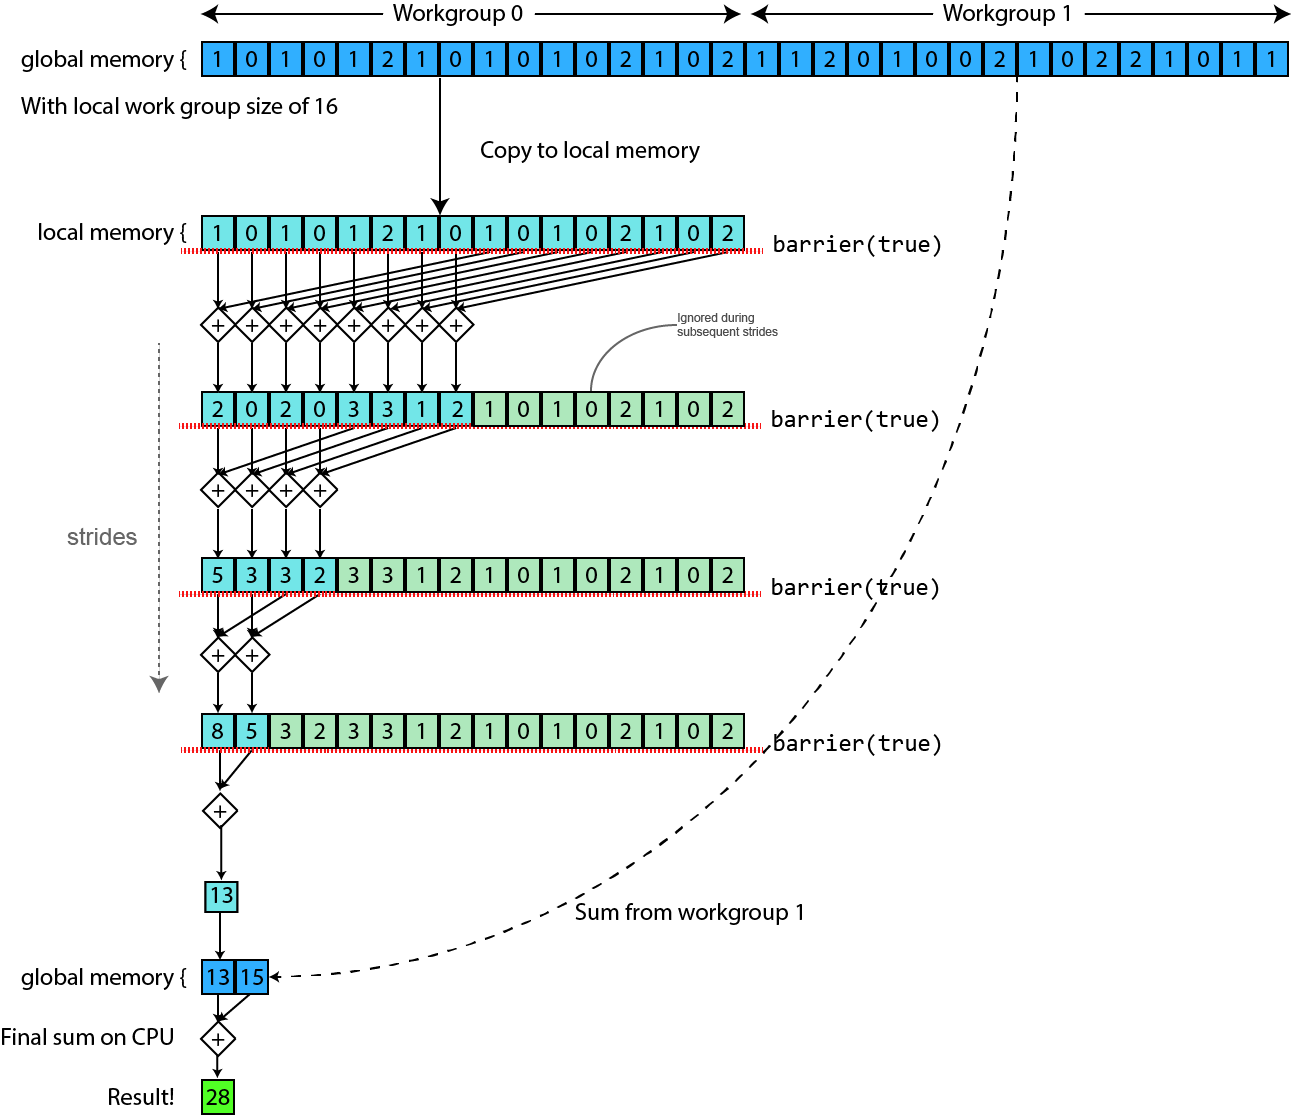
\includegraphics[width=\textwidth]{images/gpu-reduction.png}}
	\caption{Reduction algorithm with multiple local memory strides}
	\label{fig:reduction}
\end{figure}

In \ref{fig:reduction} we see a visual representation of the reduction algorithm. First we copy our data into global memory, then we pass over to the algorithm above. Once there each of the items in our work group copy the segment of data they are working on into local memory, before iteratively reducing the data in that buffer by half on each round of summation until only one value in local buffer array slot zero remains. This is then written into global memory and the final summation of these values (one for each work group) calculated on the CPU. Note that we set the local work group to size 16 in order to make it easier to show on the diagram, but in practice this value will be much larger.

Given that we are reducing by half on every iteration it is important for this algorithm that the number of work items in a work group be a power of two. This is of course not a requirement for all algorithms taking advantage of local memory.

Now let us look at the kernel, invocation and supporting function code:

\begin{lstlisting}
gpukernel 1 reduce(global val input long[], global partialSums long[], local localSums long[]){
	local_id = get_local_id(0)
	group_size = get_local_size(0)
	
	// Copy from global memory to local memory
	localSums[local_id] = input[get_global_id(0)]
	
	// Loop for computing localSums
	stride = group_size/2
	while(stride>0) {
		// Waiting for each 2x2 addition into given workgroup
		barrier(true)
		// Divide WorkGroup into 2 parts and add elements 2 by 2
		// between local_id and local_id + stride
		if (local_id < stride){
			localSums[local_id] += localSums[local_id + stride]
		}
		stride/=2
	}
	
	if(local_id == 0){ // Write result into global memory
		partialSums[get_group_id(0)] = localSums[0]
	}
}

def chooseGPUDeviceGroup(gpuDev gpus.DeviceGroup[], cpuDev gpus.DeviceGroup[]) {
	if(not gpuDev){//no gpu return first cpu
		cpuDev[0]
	}else{//intel hd graphics not as good as nvidea dedicated gpu or ati so deprioritize
		for(grp in gpuDev){
			if('Intel' not in grp.platformName){
				return grp
			}
		}
		gpuDev[0]//intel device then...
	}
}

def makeData(itemcount int, range = 3){
	data = new long[itemcount]
	
	random = new java.util.Random(654L)
	for(i = 0; i < itemcount; i++){
		data[i] = random.nextInt(range)//output: 0,1 or 2 with default range = 3
	}
	data
}

def sum(inputs long...){
	ret = 0
	for(i in inputs){
		ret += i
	}
	ret
}


def main(){
	gps = gpus.GPU()
	deviceGrp = chooseGPUDeviceGroup(gps.getGPUDevices(), gps.getCPUDevices())
	device = deviceGrp.devices[0]
	
	localItemSize = device.getMaxWorkItemSizes()[0] as int //algo requires local memory to be power of two size,
	//the max first dimention gpu size is a factor of two so we use this 
	
	InputDataSize = 1000*localItemSize as int
	System.\out.println("InputDataSize: {InputDataSize} elements")
	
	inputdata = device.makeOffHeapArrayIn(long[].class, InputDataSize)
	partialSums = device.makeOffHeapArrayMixed(long[].class, InputDataSize/localItemSize)
	localSums = gpus.Local(long[].class, localItemSize)
	data = makeData(InputDataSize)
	c1 := inputdata.writeToBuffer(data)//create some psudo random data
	
	inst = reduce(inputdata, partialSums, localSums)
	compute := device.exe(inst, [InputDataSize], [localItemSize], c1)//we must pass in the local item size for each work group
	ret = partialSums.readFromBuffer(compute)
	
	ctime = c1.getProfilingInfo().toString()
	
	//cleanup  
	del inputdata, partialSums
	del c1, compute
	del deviceGrp, device
	del inst
	
	restum = sum(ret)//sum of the partialSums in the  array slots to get our result
	verify = sum(data)//verify result on CPU
	
	System.\out.println('PASS! result: {restum}' if restum == verify else 'FAIL! result {restum} vs {verify}')
	""
}

///////////
//Output:
//InputDataSize: 1024000 elements
//PASS! result: 1024399

//Assuming execution is taking place on a gpu with the first MaxWorkItemSize elemnt of 1024 .
\end{lstlisting}

The only significant change we make here in terms of execution vs a kernel with only global memory interaction is in having to provide a local work size dimension array, in the same way as we do global dimensions - \lstinline{device.exe(inst, [ItemCount], [localItemSize], c1)}.

In the final phase of the algorithm above we are obtaining the resultant value by summing the values within the array read from our GPU. It is possible to perform this final step on the GPU but for the purposes of clarity in this example this has been excluded.

\subsection{Example Kernel using local Variables}
Let us now revisit our matrix multiplication example examined previously and see if we can improve performance by using local memory, specifically local variables...

\begin{figure}[H]
	\centerline{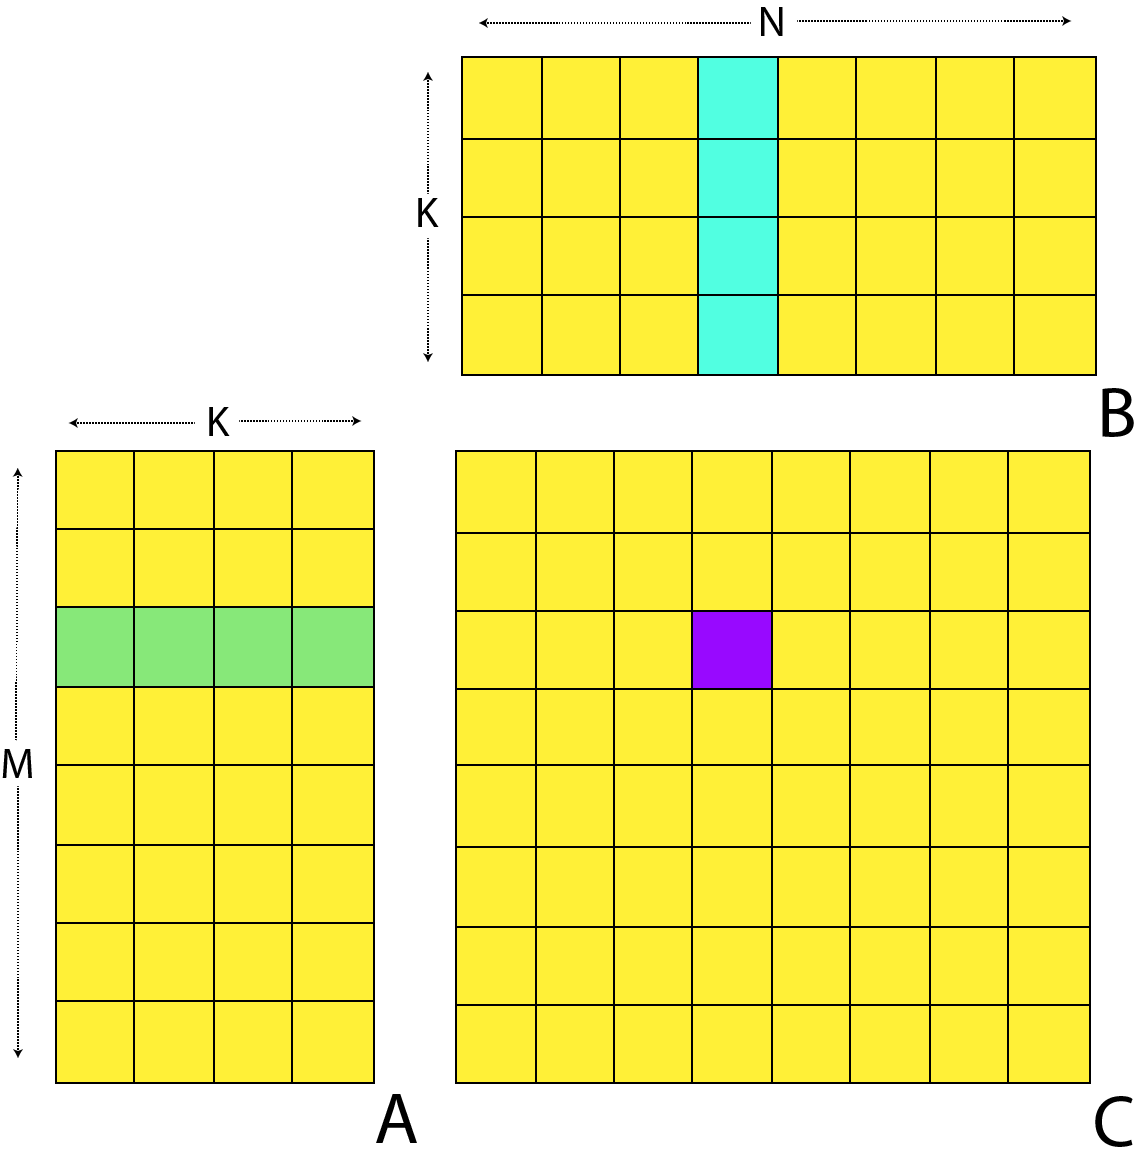
\includegraphics[width=\textwidth]{images/gpu-matmult1.png}}
	\caption{A naive algorithm for matrix multiplication}
	\label{fig:matmult1}
\end{figure}

We see in \ref{fig:matmult1} that each resulting cell is the product of each row of A and column of B summed together. We can iterate in a couple loop through each row and column of A and B respectfully. The code implementing this algorithm on the GPU and CPU is very similar and can be seen in functions \lstinline{matMultNaive} and \lstinline{matMultOnCPU}. It turns out that this algorithm expresses a high degree of spatial locality since a row of C is dependant on every value in B and a row of A, hence if we dedicate calculation of an element in C to a work item in our GPU we end up loading the values in A and B many multiples of times. In fact, relative to the amount of work done simply loading data (a relatively slow operation) we spend very little time doing actual computation.

We can improve on this algorithm by making use of a local cache as follows:

\begin{figure}[H]
	\centerline{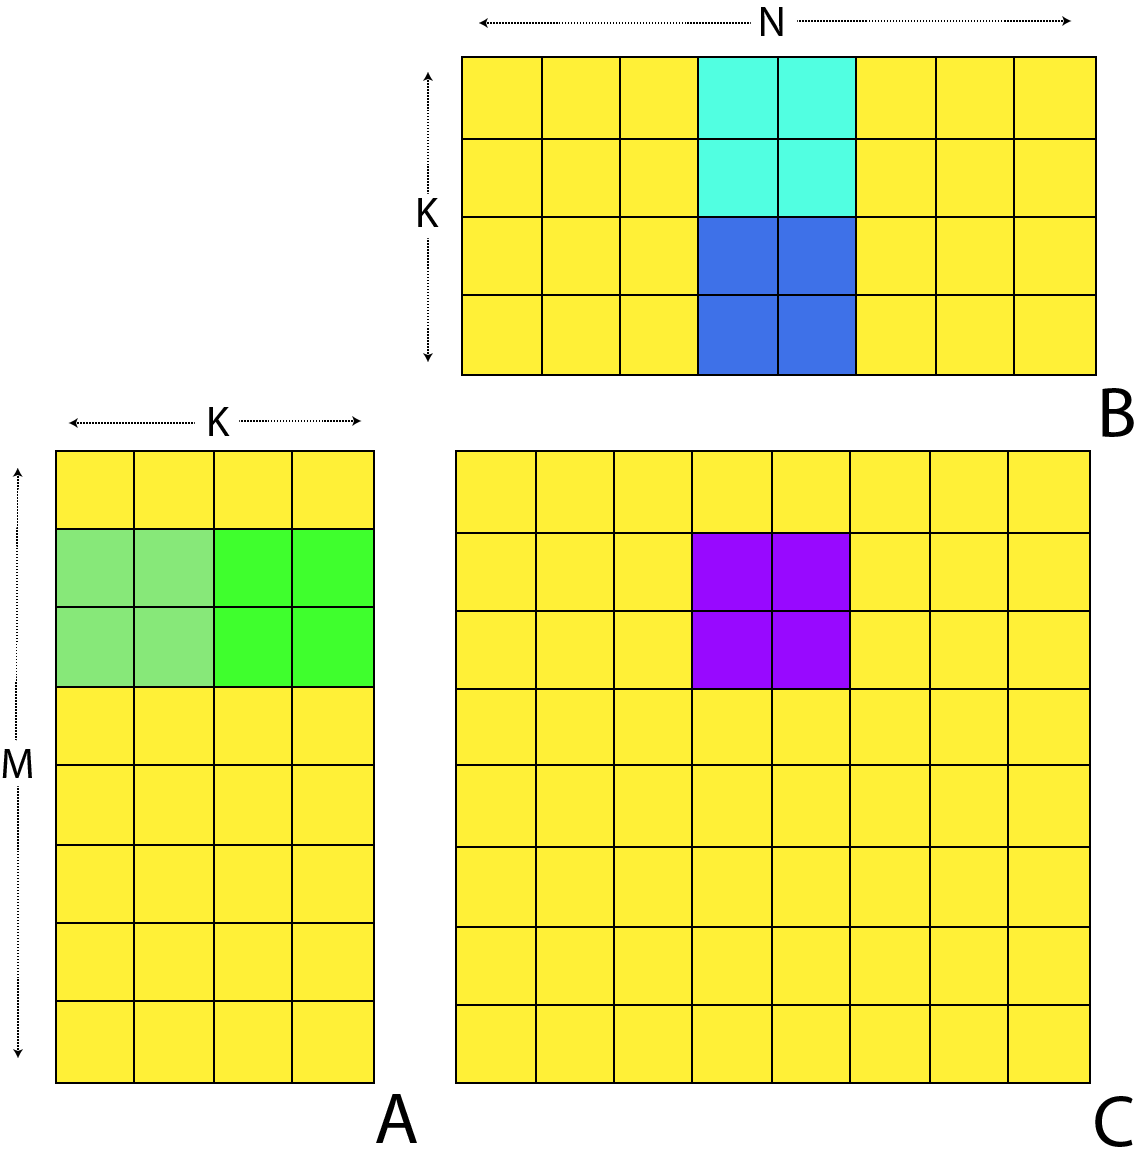
\includegraphics[width=\textwidth]{images/gpu-matmult2.png}}
	\caption{An algorithm for matrix multiplication utilizing local memory cache.}
	\label{fig:matmult2}
\end{figure}

In \ref{fig:matmult2} we see that we can calculate a block of values of C by caching in local memory two equal sized segments from A and B. The overall calculation performed by our work group is shown in \ref{fig:matmult3}:

\begin{figure}[H]
	\centerline{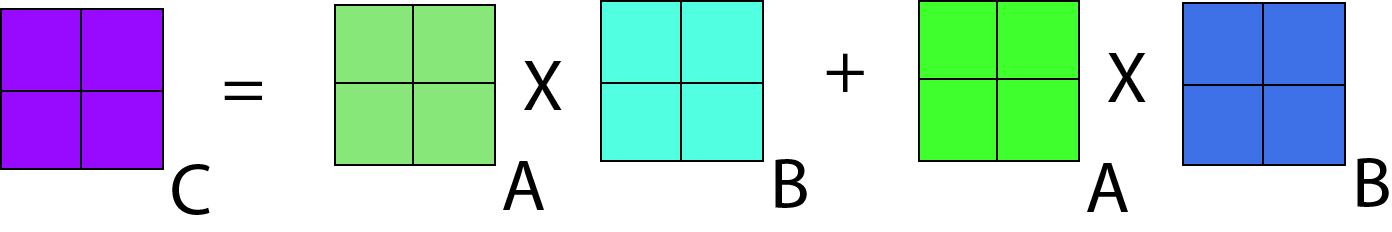
\includegraphics[width=\textwidth]{images/gpu-matmult3.png}}
	\caption{A calculation of a region of our output array C}
	\label{fig:matmult3}
\end{figure}

We can see how an individual value of C is from the local cache in \ref{fig:matmult4}.

\begin{figure}[H]
	\centerline{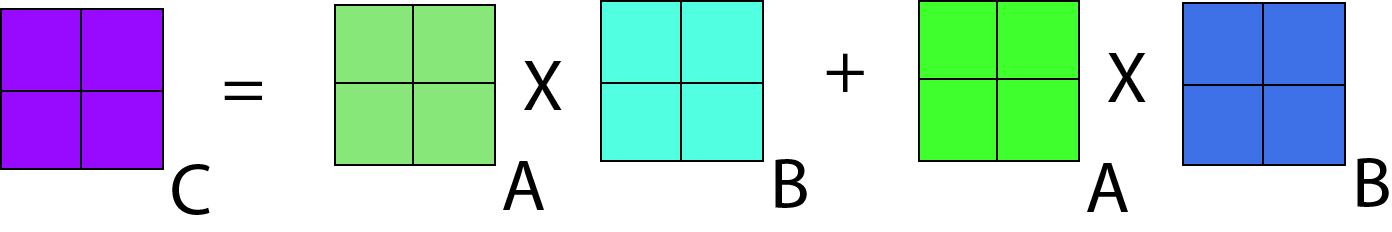
\includegraphics[width=\textwidth]{images/gpu-matmult3.png}}
	\caption{Calculation of a single element of the range in C}
	\label{fig:matmult4}
\end{figure}

Let us now look at the code which implements this, in function: \lstinline{matMultLocal}. Below the naive and cpu implementation of matrix multiplication are included for sake of comparison. We square a 128 by 128 float element matrix populated with pseudo random data:

\begin{lstlisting}
def matMultOnCPU(M int, N int, K int, A float[2], B float[2], C float[2]){
	for (m=0; m<M; m++) {
		for (n=0; n<N; n++) {
			acc = 0.f
			for (k=0; k<K; k++) {
				acc += A[k][m] * B[n][k]
			}
			C[n][m] = acc
		}
	}
}

gpukernel 2 matMultNaive(M int, N int, K int, constant A float[2], constant B float[2], global out C float[2]) {
	globalRow = get_global_id(0) 
	globalCol = get_global_id(1) 
	
	acc = 0.0f;
	for (k=0; k<K; k++) {
		acc += A[k*M + globalRow] * B[globalCol*K + k]
	}
	
	C[globalCol*M + globalRow] = acc;
}

val CacheSize = 16

gpukernel 2 matMultLocal(M int, N int, K int, constant A float[2], constant B float[2], global out C float[2]) {
	row = get_local_id(0)
	col = get_local_id(1)
	globalRow = CacheSize*get_group_id(0) + row //row of C (0..M)
	globalCol = CacheSize*get_group_id(1) + col //col of C (0..N)
	
	//local memory holding cache of CacheSize*CacheSize elements from A and B
	local cacheA = float[CacheSize, CacheSize]
	local cacheb = float[CacheSize, CacheSize]
	
	acc = 0.0f
	
	//loop over all tiles
	cacheSize int = K/CacheSize
	for (t=0; t<cacheSize; t++) {
		//cache a section of A and B from global memory into local memory tiledRow = CacheSize*t + row
		tiledCol = CacheSize*t + col
		cacheA[col][row] = A[tiledCol*M + globalRow]
		cacheb[col][row] = B[globalCol*K + tiledRow]
		
		barrier(true)//ensure all work items finished caching
		
		for (k=0; k<CacheSize; k++) {//accumulate result for matrix subsections
			acc += cacheA[k][row] * cacheb[col][k]
		}
		
		barrier(true)//ensure all work items finished before moving on to next cache section
	}
	
	C[globalCol*M + globalRow] = acc
}

def chooseGPUDeviceGroup(gpuDev gpus.DeviceGroup[], cpuDev gpus.DeviceGroup[]) {
	if(not gpuDev){//no gpu return first cpu
		cpuDev[0]
	}else{//intel hd graphics not as good as nvidea dedicated gpu or ati so deprioritize
		for(grp in gpuDev){
			if('Intel' not in grp.platformName){
				return grp
			}
		}
		gpuDev[0]//intel device then...
	}
}

def createData(xy int, range = 10){
	ret = float[xy, xy]
	random = new java.util.Random(654L)
	for(n = 0; n < xy; n++){
		for(m = 0; m < xy; m++){
			ret[n,m] = random.nextInt(range+1)//1. ... 10. inclusive
		}
	}
	ret
}

def main(){
	gps = gpus.GPU()
	cpus = gps.getCPUDevices()
	deviceGrp = chooseGPUDeviceGroup(gps.getGPUDevices(), cpus)
	device = deviceGrp.devices[0]
	
	xy = 128//assume square matrix with 128 * 128 elements
	
	matrixA = device.makeOffHeapArrayIn(float[2].class, xy, xy)
	resultNaive = device.makeOffHeapArrayOut(float[2].class, xy, xy)
	resultLocal = device.makeOffHeapArrayOut(float[2].class, xy, xy)
	
	data = createData(xy)//blocking operation
	
	matrixA.writeToBuffer(data)
	
	inst1 = matMultNaive(xy, xy, xy, matrixA, matrixA, resultNaive)
	inst2 = matMultLocal(xy, xy, xy, matrixA, matrixA, resultLocal)
	comp1 := device.exe(inst1, [xy xy], null)
	comp2 := device.exe(inst2, [xy xy], [CacheSize CacheSize])
	
	resNative = resultNaive.readFromBuffer()
	resLocal = resultLocal.readFromBuffer()
	
	conventional = float[xy, xy]
	tick = System.currentTimeMillis()
	matMultOnCPU(xy, xy, xy, data, data, conventional)
	toc = System.currentTimeMillis()
	
	System.\out.println('Time to compute on CPU: ' + (toc - tick) + "ms")
	System.\out.println('Naive ' + ('PASS ' if resNative == conventional else 'FAIL ') + comp1.getProfilingInfo())
	System.\out.println('Local ' + ('PASS ' if resLocal == conventional else 'FAIL ') + comp2.getProfilingInfo())
	
	//cleanup
	del matrixA, resultNaive, resultLocal
	del deviceGrp, device
	del inst1, inst2
	del comp1, comp2
}
\end{lstlisting}
Output when running on a single core of a Intel Core i7-3770K (quad core) CPU and 480 parallel work items of one NVIDIA GeForce GTX 570 (i.e. of a comparable generation):

\begin{lstlisting}
Time to compute on CPU: 20ms
Naive PASS Work Duration: 0.293ms
Local PASS Work Duration: 0.051ms
\end{lstlisting}

Observe that we create the local cache, local variable, within the \lstinline{matMultLocal} kernel itself instead of passing it in.

What is interesting here is the effect of our caching optimization. Armed with our profiling information (see above), we can measure the impact of this. Execution on a single core CPU takes 20 milliseconds, our naive implementation on the other hand takes 0.293 of a millisecond which is 68x quicker. We achieve a further improvement of almost 6x on this when we use local memory implementation. This brings our overall speed improvement to almost 400x over a single core CPU! Certainly worth the extra work.

Of course, there are further optimizations we can add to further increase this, and the algorithm needs to be adjusted to deal with inputs which don't divide nicely into our cache size, but for the sake of brevity we shall leave this here.

\section{Explicit memory management}
Since we are working with non heap managed memory on the GPU, and because there generally is very little of it (relative to general purpose RAM where our heap resides, and other persistent storage such as disk drives) it is impractical to offer garbage collection of it. Thus we must explicitly delete/free GPU resources either by calling the delete method on the a relevant object, or by using the del keyword. Concurnas' Garbage collection mechanism will not automatically free these resources.

The types of object which we must explicitly free one we have finished with them are:
\begin{sloppypar}
	\begin{itemize}
		\item \textbf{Buffers}: \lstinline{gpus.GPUBufferManagedInput}, \lstinline{gpus.GPUBufferManagedOutput}, \lstinline{gpus.GPUBufferManagedMixedSingle}, \lstinline{gpus.GPUBufferManagedInSingle}, \lstinline{gpus.GPUBufferManagedOutSingle}, \lstinline{gpus.GPUBufferManagedMixedSingle}. Note that Local buffers do not need deletion as they are not allocated nor allocatable outside of the GPU.
		\item \textbf{DeviceGroups}: \lstinline{gpus.DeviceGroup}
		\item \textbf{Devices}: \lstinline{gpus.Device}
		\item \textbf{Kernels}: \lstinline{gpus.Kernel}
		\item \textbf{GPURefs}: Returned from asynchronous non blocking calls from: 
		\begin{itemize}
			\item All Buffer memory interaction functions.
			\item Device kernel execution \lstinline{Device.exe(...)}
		\end{itemize}
	\end{itemize}
\end{sloppypar}

In the case of GPURefs. If one deliberately negates or forgets to capture the resultant GPURef from an asynchronous non blocking GPU call then in addition to the calling code waiting for the call to complete (thus turning the call into a blocking call), the delete method will be called on the GPURef upon completion, thus freeing the memory allocated to manage the ref. This is a deliberate and very convenient mechanism for avoiding memory leaks.

This can be achieved either by explicitly calling the delete method on these objects, or by using the del keyword.
\begin{lstlisting}
device.delete()
del deviceGroup, kernel
\end{lstlisting}

\section{Finishing}
It can be useful to explicitly wait for a device to finish all current queued execution (buffer reading, writing, kernel execution), the finish method can be invoked for this purpose which will block until all work has been completed:
\begin{lstlisting}
device.finish()
\end{lstlisting}

Calling del on a device will also implicitly call finish, thus ensuring that all work on the device has been completed before being freed.

\section{Double Precision}
Concurnas permits the use of single (float) and double (double) precision floating point types in gpu kernels and gpu functions\footnote{Normally, OpenCL implementations require an explicit declaration to perform operations on data of double precision type. But in Concurnas this is provided automatically, no explicit declaration is needed.}. It should be noted however that operations  performed on double precision type are considerably slower than the equivalent with float type. Thus when possible one should strive to use floating point type over double.

When creating arrays care should be taken to explicitly declare floating point values as float as the default instantiation type for a floating point literal values is double.

\section{Concurrent use of GPUs}
The GPU interaction related classes under \lstinline{com.concurnas.lang.gpus} (including, buffers, device groups, devices, kernels and gpurefs) are marked as transient.This is deliberate as it prevents accidental sharing of gpu related objects between differing iso's, which, if permitted would make state management challenging in most systems. It also avoids problems with attempting to persist gpu objects off heap, which doesn't make sense for gpu interaction objects.

In cases where multiple iso's require access to the GPUs at the same time, using an actor is advised, this permits one a fine degree of control over the GPUs available both from the perspective of pipelining of requests to them, and from the perspective of easily managing memory.

\section{Notes}
The reader who is aware of the inner workings OpenCL will no doubt find many aspects of the structure of the Concurnas implementation of GPU computing very familiar. This is deliberate. By not deviating to far away from "the way things are done" currently with the API exposed in raw OpenCL we hope to make GPU computing something which is natural to do for both OpenCL veterans, whilst simplifying the implementation details enough to make working with GPU's easy for newcomers.

Additionally, in the interests portability, we have omitted the tools and techniques exposed in OpenCL from version 2.0 onwards due, mainly to lack of compatibility with NVidia drivers, which for most of the older GPUs are only OpenCL 1.2 compliant.

\end{document}